\subsubsection{Quick Sort}
Quicksort is an efficient comparison sort that uses a divide and conquer algortihm. The algoritm works by chosing a pivot point, then dividing the list into two lists and based on thier value compared to the pivot point. All values less then the pivot point goes into a list usually named left, and all values equal or higher then the pivot point goes into a list usually called right. The pivot point can be choosen in many different ways, but the recommended way is to take three random indexes and take the median. After the list have been split into left and right, those are then sent into the same function where they are divided until there is only one value left. Then the value is returned and the list is concatenated left, pivot point and right.
\\[11pt]
While performing the sort the algoritm we wrote also stores the state of steps that we picked. This is done for the solution checker to be able to check if the student has drawn the correct answer when simulating the quicksort algorithm.
\begin{itemize}
    \item Initial: The initial step is stored before the sorting starts. It contains a copy of the unsorted array.
    \item Split: The split step is stored each time the algorithm splits a list, it will store the unsorted list that it will split, the pivot point, left and right list.
    \item Merge: The merge step is stored each time the algorithm merges the sorted lists and pivot point. It will store information about the sorted left and right list, the pivot point and the sorted list after the merge.
\end{itemize}
\begin{figure}
    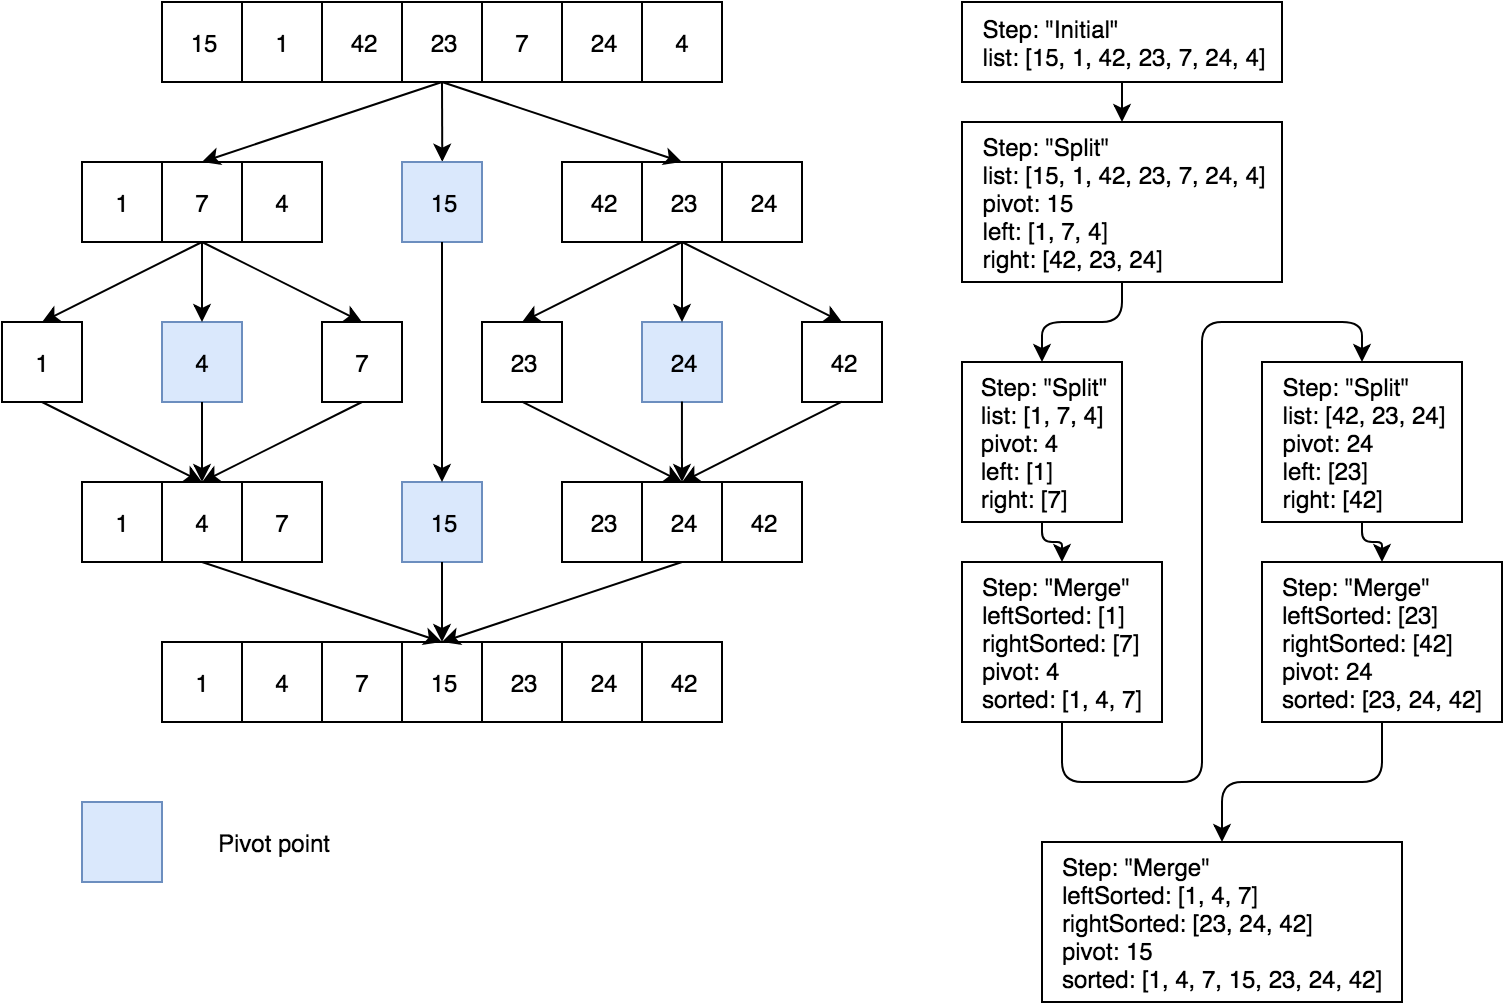
\includegraphics[width=\linewidth]{/diagrammer/Quicksort}
    \caption{Quicksort}
    \label{fig:quicksort}
\end{figure}